\chapter{營隊介紹}
\chapterauthor{熊熊兔兔}

\section{營隊規定}


\subsection{要遵守的規定}
\begin{enumerate}[label=\arabic*)]
\item 營隊時間為8/13$\sim$8/15 08:00$\sim$16:00 8/16 08:00$\sim$\underline{\textbf{19:00}},時間內請遵守一切規定與指示。
\item 活動範圍皆在科教館內,除非在隊輔指示下,否則禁止出館。
\item 部分大型活動會在武陵大陸上舉行,但請勿進入教學區(就是有教室的地方)。
\item 身體若有任何不適,立即通知身旁的隊輔。
\item 隨時攜帶名牌,否則須做勞動服務協助本營。
\item 你們身旁的隊輔皆為科學班的電神,盡量問他們問題吧!
\item 認真上課,這是非常難得的機會,我們篩掉了很多人,請自重。
\end{enumerate}

\subsection{認真要遵守的規定}
\begin{enumerate}[label=\arabic*)]
\item 各位是從異世界被選中的學員,科學班遭遇了空前的危機,維持和平的條約消失了!(熊熊:喔不!!!!)
\item 在這幾天的營隊中,在課程或活動後會頒發部分線索,最後獲得最多線索點數的小隊將成為優勝。
\item 線索會與所有本部之人分享,希望諸位能幫助科學班解決危機。
\item 各個小活動與最終任務皆有獎項,爭取優勝小隊的同時別忘記認真參與各活動與課程。(需事先閱讀最終遊戲之規則。)(兔兔:在倒數第二章喔)
\end{enumerate}
\newpage
\subsection{活動範圍}
主要的活動範圍都在科教館,請注意,育菁樓附近正在興建新大樓,請勿從施工區穿越,請走育菁樓及崇德樓中間的走道抵達科教館。
\begin{center}
\begin{figure}[H]
\centering
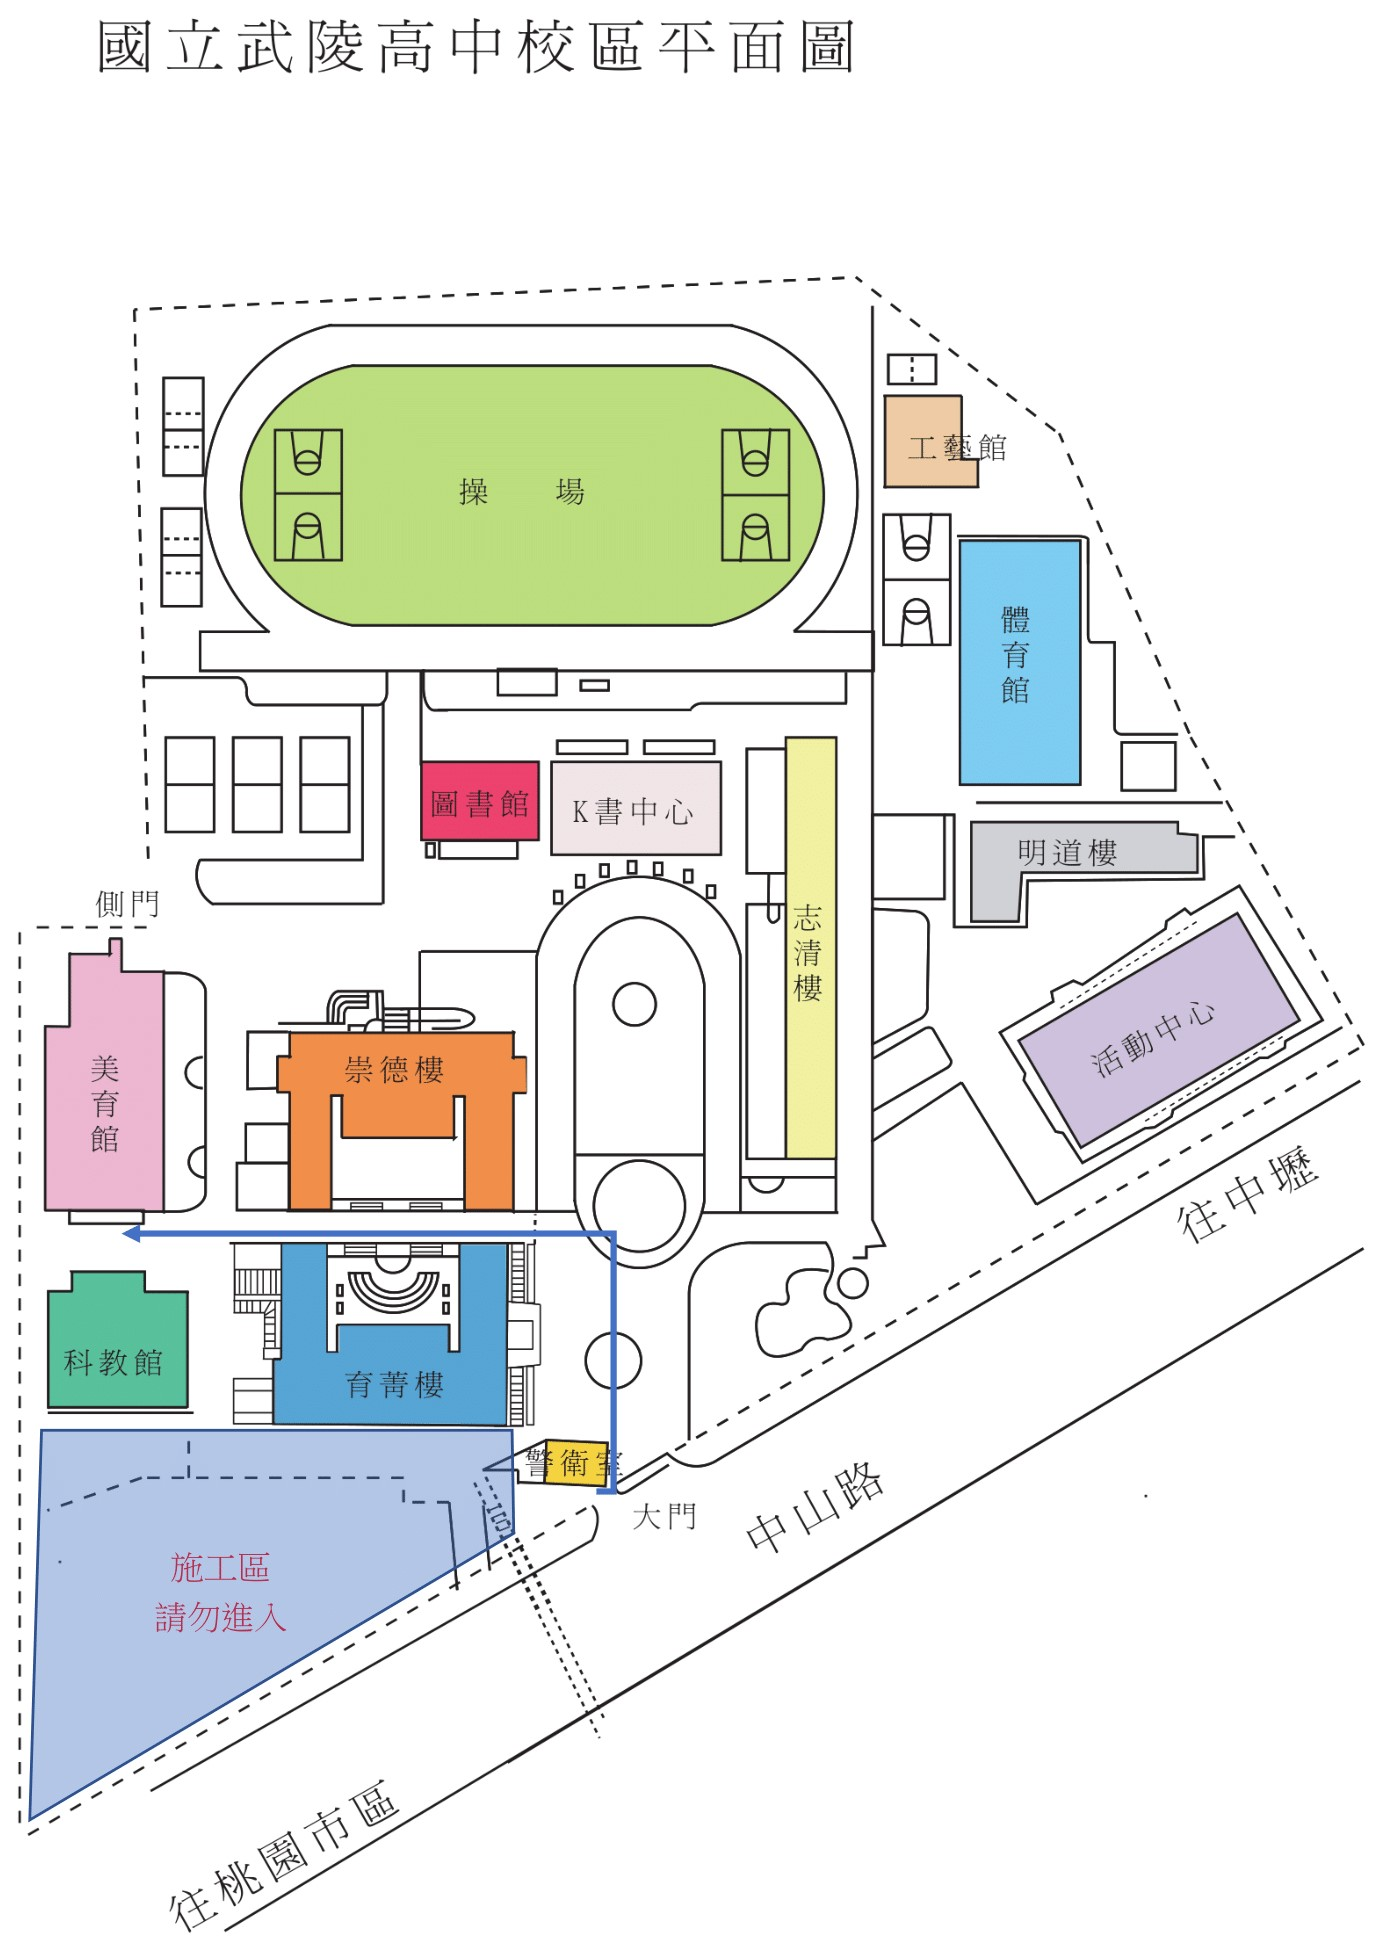
\includegraphics[width=15cm, center]{map.jpg}
\end{figure}
\end{center}
\section{日程}
\begin{table}[H]
\centering
\resizebox{10cm}{!}{%
\begin{tabular}{|c|c|c|}
\hline
\textbf{時間} & \multicolumn{2}{c|}{\textbf{8/13(二)}} \\ \hline
\textbf{8:00$\sim$8:50} & \multicolumn{2}{c|}{We Want You!} \\ \hline
\textbf{8:50$\sim$9:00} & \multicolumn{2}{c|}{Break} \\ \hline
\textbf{9:00$\sim$9:50} & \multicolumn{2}{c|}{武陵爭鬥的開端} \\ \hline
\textbf{9:50$\sim$10:00} & \multicolumn{2}{c|}{Break} \\ \hline
\multirow{4}{*}{\textbf{10:00$\sim$12:00}} & \multicolumn{2}{c|}{\multirow{4}{*}{真$\cdot$能力傳承}} \\
 & \multicolumn{2}{c|}{} \\
 & \multicolumn{2}{c|}{} \\
 & \multicolumn{2}{c|}{} \\ \hline
\textbf{12:00$\sim$12:30} & \multicolumn{2}{c|}{Lunch} \\ \hline
\textbf{12:30$\sim$12:55} & \multicolumn{2}{c|}{Nap} \\ \hline
\textbf{13:05$\sim$13:55} & \begin{tabular}[c]{@{}c@{}}我的改變\\ 你看的見\end{tabular} & 雪豹好可愛 \\ \hline
\textbf{13:55$\sim$14:05} & \multicolumn{2}{c|}{Break} \\ \hline
\textbf{14:05$\sim$14:55} & \multicolumn{2}{c|}{生輔} \\ \hline
\textbf{14:55$\sim$15:05} & \multicolumn{2}{c|}{Break} \\ \hline
\textbf{15:05$\sim$15:55} & 雪豹好可愛 & 所以…行! \\ \hline
\textbf{16:00$\sim$} & \multicolumn{2}{c|}{Home} \\ \hline
\end{tabular}%
}
\end{table}
% Please add the following required packages to your document preamble:
% \usepackage{multirow}
% \usepackage{graphicx}
\begin{table}[H]
\centering
\resizebox{\textwidth}{!}{%
\begin{tabular}{|c|c|c|c|c|c|c|}
\hline
\textbf{時間} & \multicolumn{2}{c|}{\textbf{8/14(三)}} & \multicolumn{2}{c|}{\textbf{8/15(四)}} & \multicolumn{2}{c|}{\textbf{8/16(五)}} \\ \hline
\textbf{08:00$\sim$08:15} & \multicolumn{6}{c|}{肌動蛋白的磷酸化與Z線的移動造成肝中丙酮酸再造} \\ \hline
\textbf{08:15$\sim$08:25} & \multicolumn{6}{c|}{Break} \\ \hline
\textbf{08:25$\sim$09:15} & \multicolumn{2}{c|}{\multirow{3}{*}{溶解度與克氏循環}} & 急急護法現身 & 幾何幾何? & 所以…行! & 焓是長來幹嘛的? \\ \cline{1-1} \cline{4-7} 
\textbf{09:15$\sim$09:25} & \multicolumn{2}{c|}{} & \multicolumn{4}{c|}{Break} \\ \cline{1-1} \cline{4-7} 
\textbf{09:25$\sim$10:15} & \multicolumn{2}{c|}{} & \multicolumn{2}{c|}{1A2B} & \multicolumn{2}{c|}{你該知道的事} \\ \hline
\textbf{10:15$\sim$10:20} & \multicolumn{6}{c|}{Break} \\ \hline
\textbf{10:20$\sim$11:10} & 霧裏看物理 & 急急護法現身 & \multicolumn{2}{c|}{\multirow{2}{*}{分身!!!!!}} & \multicolumn{2}{c|}{\multirow{2}{*}{波濤洶湧}} \\ \cline{1-3}
\textbf{11:10$\sim$12:00} & 幾何幾何? & \begin{tabular}[c]{@{}c@{}}我的改變\\ 你看的見\end{tabular} & \multicolumn{2}{c|}{} & \multicolumn{2}{c|}{} \\ \hline
\textbf{12:00$\sim$12:30} & \multicolumn{6}{c|}{Lunch} \\ \hline
\textbf{12:30$\sim$12:55} & \multicolumn{6}{c|}{Nap} \\ \hline
\textbf{13:05$\sim$13:55} & 焓是長來幹嘛的? & 霧裏看物理 & \multicolumn{2}{c|}{\multirow{5}{*}{時空裂縫}} & \multicolumn{2}{c|}{\multirow{3}{*}{武陵大陸的終章}} \\ \cline{1-3}
\textbf{13:55$\sim$14:05} & \multicolumn{2}{c|}{Break} & \multicolumn{2}{c|}{} & \multicolumn{2}{c|}{} \\ \cline{1-3}
\textbf{14:05$\sim$14:55} & \multicolumn{2}{c|}{\multirow{3}{*}{胖子與NaOH}} & \multicolumn{2}{c|}{} & \multicolumn{2}{c|}{} \\ \cline{1-1} \cline{6-7} 
\textbf{14:55$\sim$15:05} & \multicolumn{2}{c|}{} & \multicolumn{2}{c|}{} & \multicolumn{2}{c|}{Break} \\ \cline{1-1} \cline{6-7} 
\textbf{15:05$\sim$15:55} & \multicolumn{2}{c|}{} & \multicolumn{2}{c|}{} & \multicolumn{2}{c|}{The end?} \\ \hline
\textbf{16:00$\sim$} & \multicolumn{2}{c|}{Home} & \multicolumn{2}{c|}{Home} & \multicolumn{2}{c|}{\begin{tabular}[c]{@{}c@{}}16:00$\sim$19:00 \\ Final\end{tabular}} \\ \hline
\end{tabular}%
}
\end{table}
\section{小隊員\&隊輔}
% Please add the following required packages to your document preamble:
% \usepackage{graphicx}
\begin{table}[H]
\centering
\resizebox{\textwidth}{!}{%
\begin{tabular}{|c|c|c|c|c|c|c|c|c|}
\hline
\textbf{小隊} & \multicolumn{6}{c|}{\textbf{隊員}} & \multicolumn{2}{c|}{\textbf{隊輔}} \\ \hline
1 & 葉書佑 & 李澤暘 & 楊芷菱 & 游聿堂 & 童靖幃 & 蔡品昱 & 黃芃嫣 & 黃智笙 \\ \hline
2 & 羅大剛 & 許珍瑋 & 黎廷緯 & 陳思妤 & 林詩耕 & 許育晟 & 邱柏偉 & 葉欲禾 \\ \hline
3 & 周宇凡 & 林哲安 & 江伯翊 & 黃昱昇 & 黃柏瑜 & 楊瑄芸 & 鄧駿樺 & 柳凱馨 \\ \hline
4 & 林奕杉 & 陸柏蓉 & 林立恩 & 祁幃凱 & 林沅龍 & 李家勝 & 張智閎 & 蘇郁棻 \\ \hline
5 & 黃子倫 & 林佑瑋 & 呂紹頡 & 洪鈺翔 & 呂丞凱 & 吳奕萱 & 戴佑丞 & 鄧朝語 \\ \hline
6 & 李瑞恩 & 車亮萱 & 楊心澄 & 謝廷承 & 陳威廷 & 吳宇凡 & 林陽 & 胡睿喆 \\ \hline
7 & 徐震閎 & 林澄 & 柯儀寀 & 吳宇平 & 汪煒翔 & 吳孟學 & 蔡博恩 & 賴城諭 \\ \hline
\end{tabular}%
}
\end{table}
\section{積分表與積分表}
\begin{table}[H]
\begin{minipage}{0.5\linewidth}
\centering
\begin{tabular}{|c|c|c|}
\hline
時間點 & 獲得物 & 積分 \\ \hline
各課程優勝 & 小線索 & 15 \\ \hline
科教館裡藏的 & 線索碎片 & 5 \\ \hline
\multirow{2}{*}{1A2B 優勝} & 小線索 & 15 \\ \cline{2-3} 
 & 中線索 & 25 \\ \hline
\multirow{2}{*}{時空裂縫中} & 中線索 & 25 \\ \cline{2-3} 
 & 大線索 & 40 \\ \hline
\multirow{2}{*}{你該知道的事} & 小線索 & 15 \\ \cline{2-3} 
 & 中線索 & 25 \\ \hline
End Game & \multicolumn{2}{c|}{獨立計算} \\ \hline
\end{tabular}
\captionof{table}{積分表}
\end{minipage} \hfill
\begin{minipage}{0.45\linewidth}
\centering
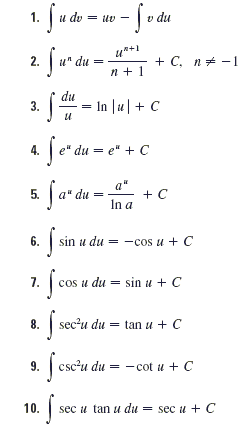
\includegraphics[width=\linewidth]{integral.png}
\captionof{figure}{積分表}
\label{fig:integral}
\end{minipage}
\end{table}

